\chapter{Fundamentação Teórica}

Nesse capítulo apresentamos uma breve introdução sobre as abstrações de
processos e os vários temas que orbitam tal conceito (threads, \emph{fork},
representação na memória, virtualização, dentre outros). Apresentamos conceitos
que são \textbf{indiretamente} ligado as abstrações de processos e que por isto
não são habitualmente explicitados na bibliografia padrão, desse modo,
evidenciar as relações entre os diferentes conceitos é extremamente útil para a
o contexto das ideias apresentadas nesse trabalho. Vale observar que a maioria
dos conceitos apresentados nessa seção baseiam-se em sistemas Unix e no padrão
POSIX. Em resumo, a proposta desse capítulo é fornecer as informações básicas
para a assimilação das ideias apresentadas neste texto.

\label{cap:fundamentacao-teorica}

\section{Processos e Threads}
\label{sec:processos-e-threads}

Normalmente programas são escritos em uma linguagem de programação específica
(e.g.; C/C++, Java, Python, Ruby, etc) e posteriormente convertidas para um
conjunto de instruções que uma máquina é capaz executar. O código fonte de uma
aplicação é representado como um ou mais arquivos que é armazenado em uma
memória \emph{não-volátil} (e.g,; disco rígido), por sua vez, este pode ter uma
relação com um ou mais arquivos executáveis (binários) gerados a partir do
fonte. O arquivo binário tem um conjunto de metadados \footnote{Descrição ou
conjunto de características de um dado ou de um item} no seu começo que auxilia
o SO a executar de forma correta um programa, tais informações são inseridas
pelo compilador e são conhecidas como \emph{headers}. Dado esse contexto, o SO
carrega o executável do disco para a memória com o objetivo de criar um novo
processo; em seguida o SO realiza a leitura dos metadados dentro do binário e
utiliza tais informações para criar os segmenos de memórias pertencentes aos
processos. Cada pedaço da memória tem um propósito específico que habilita
o SO a gerir o processo.

\begin{figure}[!h]
  \centering
  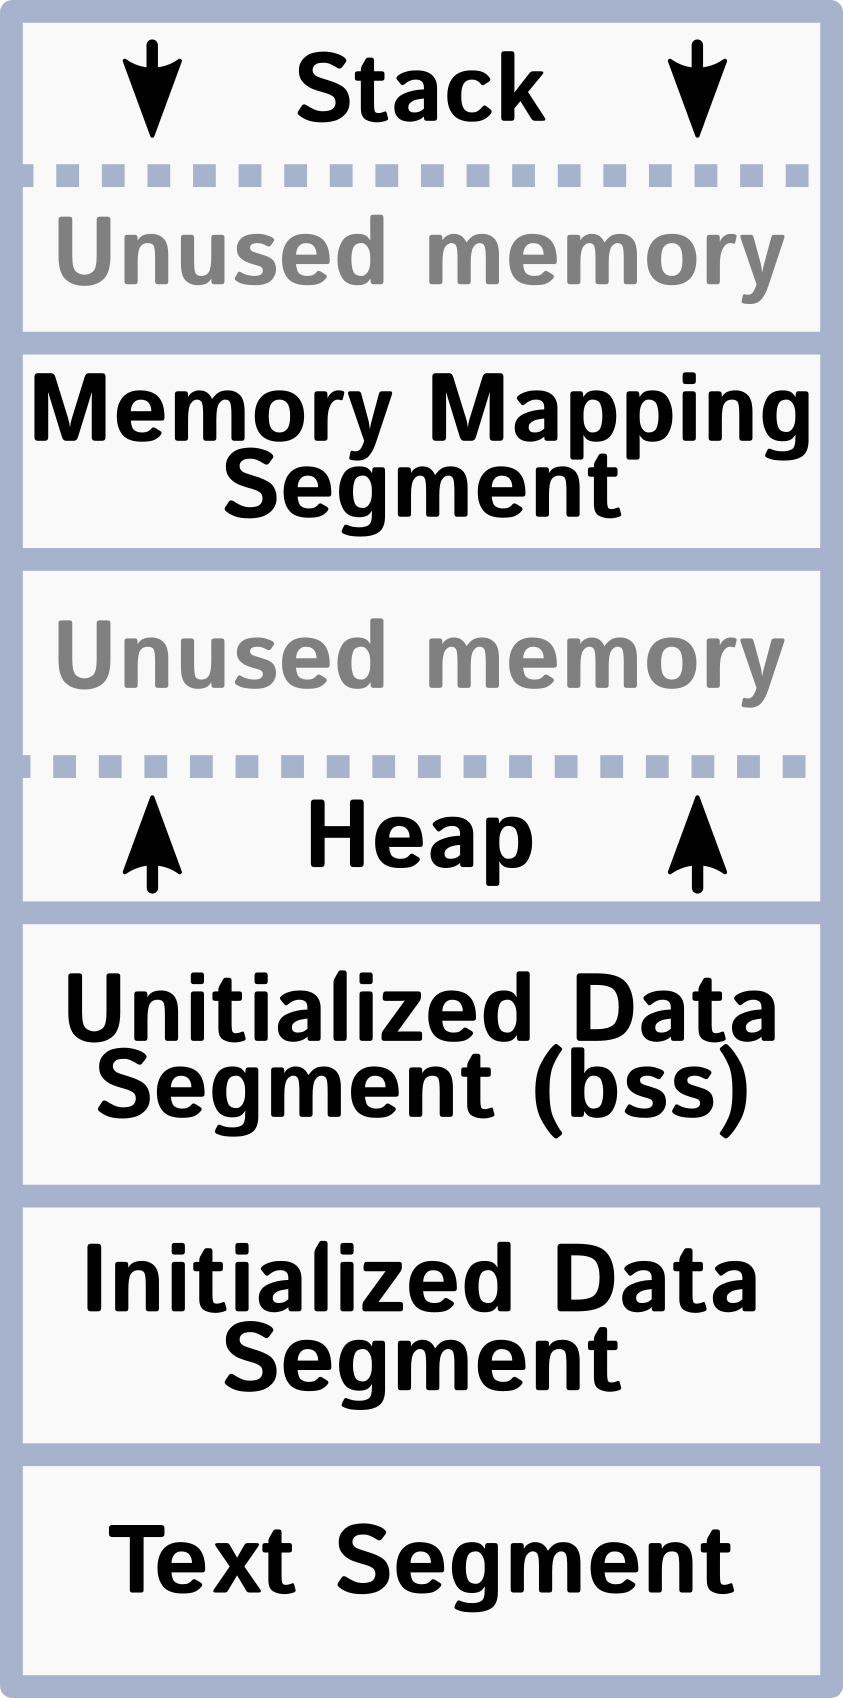
\includegraphics[width=.20\textwidth]{memory_segment} 
  \caption{Segmento de memória}
  \label{fig:memory_segment} 
\end{figure}

A Figura \ref{fig:memory_segment} ilustra seis segmentos de memória diferentes
representando o \emph{layout} de um processo após a criação dele por parte do
SO. O \textbf{segmento de texto} (\emph{Text Segment}) representa a região da
memória que mantém o código executável (compartilhável e que é somente
leitura). Já o \textbf{segmento de dados inicializáveis} (\emph{Initialized
Data Segment}) é responsável por manter variáveis estáticas, enquanto o
\textbf{segmento de dados não inicializados} (\emph{Uninitialized Data
Segment}) mantém variáveis estáticas não inicializadas.  Vale observar que o
segmento de dados não inicializável também é comumente conhecido como
\emph{Block Started by Symbol (BSS)} por causa de um antigo operador usado
pelos montadores \cite{gdb}. O \textbf{segmento de Mapeamento de Memória}
(\emph{Memory Mapping Segment}) é a região na qual o SO mapeia arquivos
diretamente na memória (e.g.; bibliotecas dinâmicas ou arquivos especificados
pelo programador). O \textbf{segmento da Stack} compreende aos dados usados
pelo programa durante a execução, como por exemplo, valores de parâmetros de
função, endereço de retorno e variáveis locais (dados temporários)
\cite{silberschatz}.  Por fim, o \textbf{segmento do Heap} mantém a memória
dinâmicamente alocada durante a execução do programa; repare que o \emph{stack}
e o \emph{heap} estão em lados oposto da memória.

O primeiro passo realizado pelo SO quando ele lê o arquivo executável é olhar
para o \emph{header} e obter as informações sobre o tamanho do segmento de
texto e dados. Em seguida, com base nas informações obtidas do \emph{header}, o
SO cria um novo espaço de endereçamento (\emph{Address Space}) com tamanho de
memória suficiente para os segmento de texto e dados. Após alocar memória, o
próximo passo consiste em copiar toda a região de código e dados lidas do
arquivo binário para a memória recém alocada; complementarmente, é feita a
inicialização de todos os registradores e os devidos ajustes no \emph{stack
pointer}. O processo tem o seu \emph{Program Counter} (PC) ajustado para a
função \emph{main} do programa \cite{patterson}, por fim, o SO insere o novo
processo na fila do escalonador. Vale a pena observar que a noção de
\textbf{Virtual Address Space (VAS)} é diretamente associada ao endereço físico
de memória atribuído a um novo processo e que por isso um processo não deve
ter conhecimento sobre outras VAS pertencentes a outros processos.

\begin{figure}[!h]
  \centering
  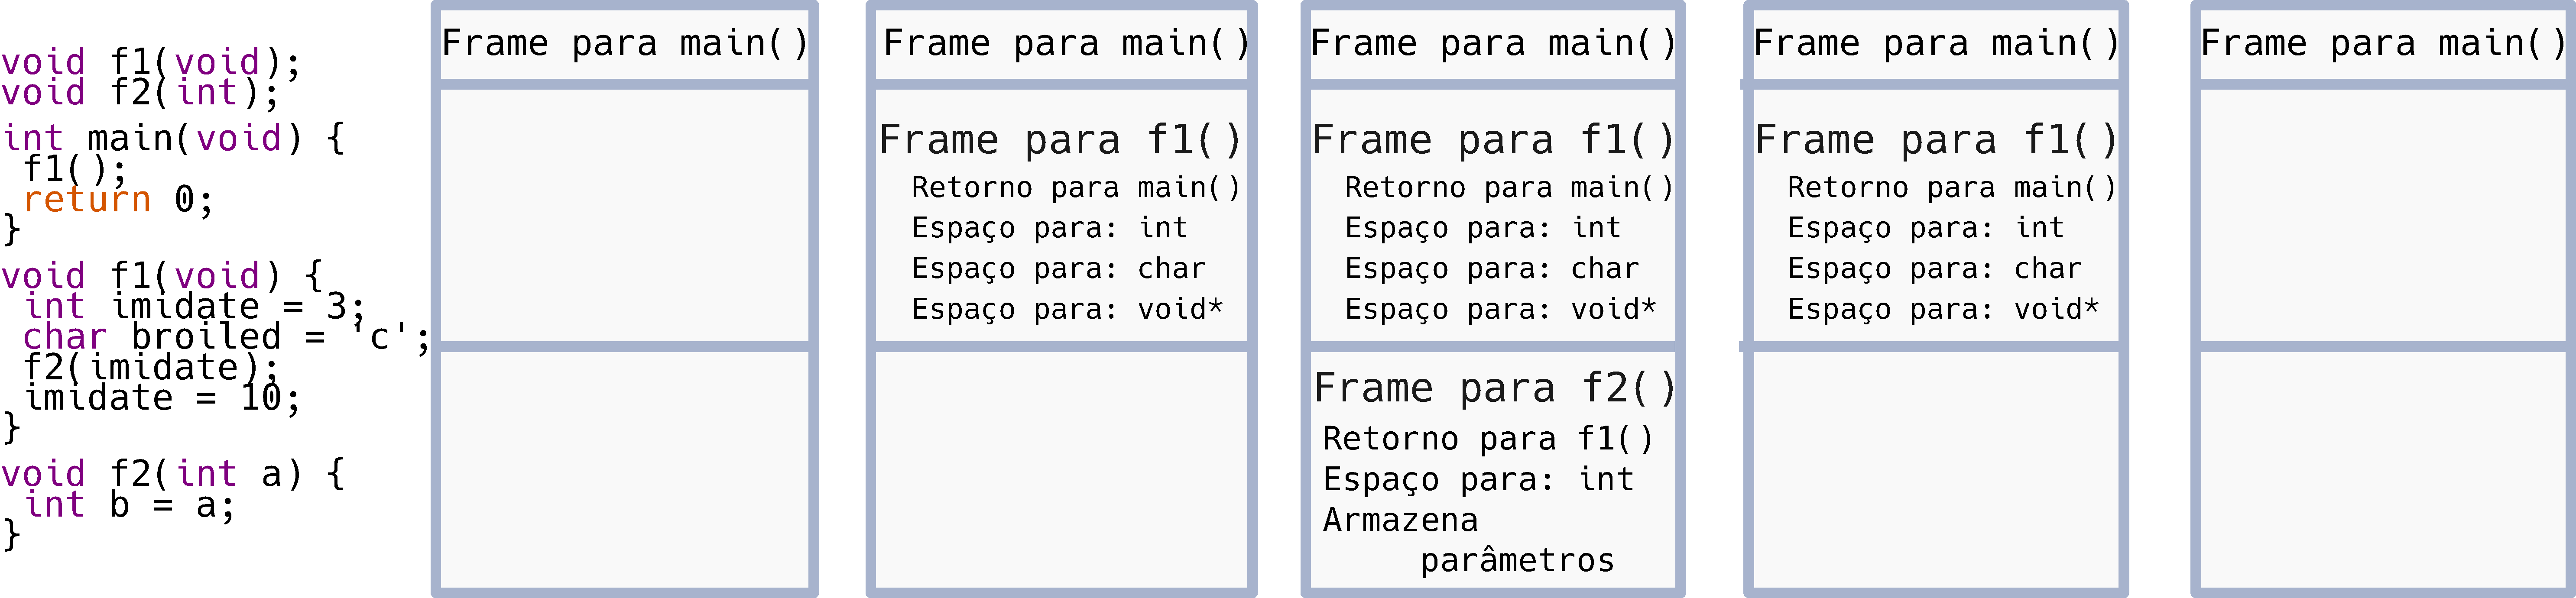
\includegraphics[width=\textwidth]{stack_frame}
  \caption{Stack frames, imagem baseada em \cite{patterson}}
  \label{fig:stack_frames} 
\end{figure}

A \emph{stack} é organizada em uma coleção de \textbf{Stack Frames}. Toda vez
que uma função é chamada ela cria um novo \emph{frame} que mantém as variáveis
locais, argumentos e o ponto de retorno relacionado a função. Um processo pode
invocar um grande número de funções durante a sua execução, consequentemente,
cada função chamada recebe um \emph{stack frame}. A Figura
\ref{fig:stack_frames} ilustra a alocação e desalocação de um simples programa
\cite{gdb}. No começo, só existe um \emph{stack frame} associado no topo da
função \texttt{main}. Quando uma função local é chamada, o SO vai alocar um
novo \emph{stack frame} no topo do \emph{frame} da \texttt{main}, esse
procedimento permite que a execução do processo ocorra de forma consistente. No
fim da execução da função, ela retorna para o ponto na qual a função foi
invocada e o processo de echer e esvaziar a \emph{stack} continua.

Todo os processos são descritos por meio de uma estrutura de dados chamado
\textbf{Process Control Block (PCB)} que é responsável por manter informações
sobre o status do processo, \emph{program counter} (PC), registradores da CPU,
informações sobre escalonamento, dados sobre contas de usuários, status de
operações de I/O e assim por diante \cite{silberschatz}. Uma dos principais
motivos para a PCB existir é o conceito de \textbf{troca de contexto} que é
responsável por colocar e tirar processos para executar em uma CPU. Por
exemplo, se o usuário tem vários processos rodando ao mesmo tempo, o SO tem que
mudar entre todos eles para que todos tenham a oportunidade de executar por um
intervalo de tempo. O SO realiza o processo de troca em duas etapas gerais: (1)
salva a PCB atual do processo e (2) carrega a PCB do outro processo. Em
poucas palavras, a troca de contexto tem que ser rápida uma vez que esta não
faz nenhum processamento considerado útil.

%TODO: Esse parágrafo é importante e está ruim. Essa discussão tem que virar
% uma seção no futuro e explorar bem a questão do isolamento e os seus tradoffs

O conceito apresentado acima revela uma característica de isolamento associada
com a forma na qual os processos funcionam; normalmente, segurança e
estabilidade são positivamente afetadas pelo isolamento de processos. Por outro
lado, existem situações que exigem que os processos cooperem entre si e nesses
casos é possível notar algumas das desvantagens inerentes a estratégia de
processos atual. Para resolver parte desse problema, algumas bibliotecas ou
chamadas de sistemas são fornecidas como uma interface para coordenar a
interação entre processos executando concomitantemente, esses são conhecidos
pelo nome de \textbf{Interprocess Communication} (IPC). Por exemplo,
desenvolvedores podem utilizar IPC para compartilhar daddos, melhorar o
desempenho das aplicações, modularidade ou por alguma questão de conveniência
em suas aplicações. O IPC tem três limitações princípais: elevam o consumo de
memória, adicionam sobrecargas extras de comunicação e tem uma certa
complexidade para serem implementadas. Essas limitações são proibitivas em
aplicações com grande demanda computacional.

\begin{figure}[!h]
  \centering
  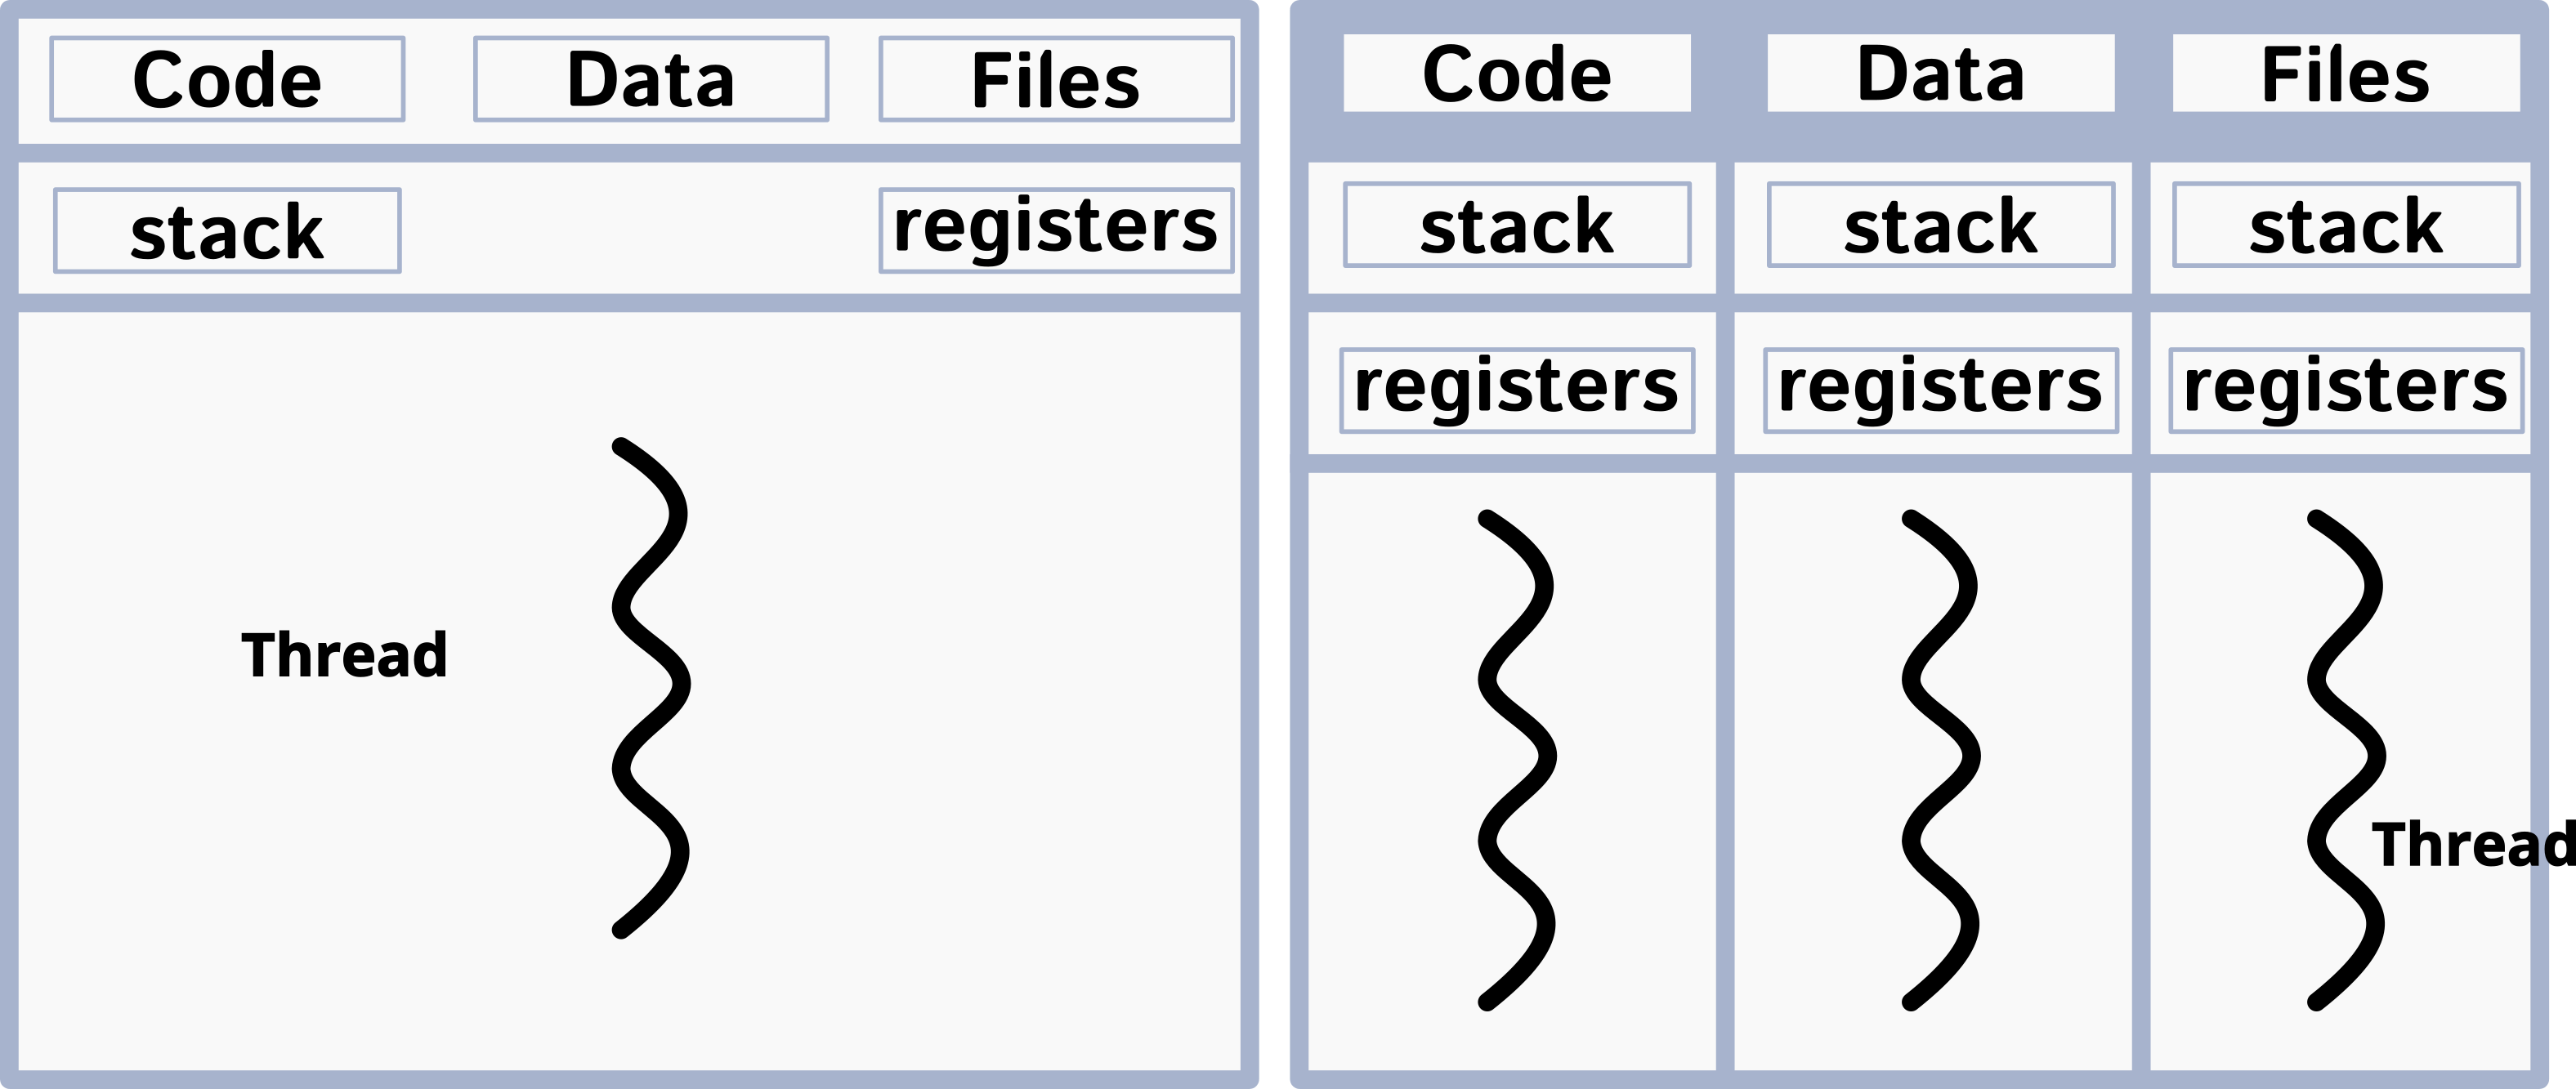
\includegraphics[width=.7\textwidth]{process_and_threads.png}
  \caption{Única thread e multi-thread, imagem baseada em \cite{silberschatz}}
  \label{fig:single_thread_multi_thread}
\end{figure}

Como é possível perceber, processos são abstrações poderosas com algumas
limitações, princípalmente ao que se refere ao desempenho e complexidade. Além
disso, processos tem apenas uma \emph{thread} para realizar todo o trabalho e
naturalmente os desenvolvedores buscam atingir mais paralelismo ou concorrência
por meio de IPC; contudo os programadores tem que lidar com as sobregargas
extras impostas por essa estratégia. Por esse motivo, buscou-se por muito tempo
por formas de elevar o desempenho das aplicações por meio de melhorias no grau
de paralelismo. Como resultado direto de tal esforço sugiu o conceito de um
processo ter multiplas \emph{threads} compartilhando práticamente todos os
elementos básicos com execessão da \emph{stack} e do PC. A Figura
\ref{fig:single_thread_multi_thread} mostra um processo com uma \emph{thread} e
outro com multiplas \emph{threads}, note na figura o isolamento da \emph{stack}
e do PC.

\lstinputlisting[
                 language=C,
                 caption={Exemplo simple de threads},
                 label={lst:simplethreads}
                ]{code/simpleThread.c}

\begin{lstlisting}[frame=single,
                   language=bash,
                   caption={Saída do exemplo de threads},
                   label={lst:simpleThreadOutput}]
$ ./example 
Thread 1 
Thread 2
$ ./example
Thread 2 
Thread 1
\end{lstlisting}

O Código \ref{lst:simplethreads} ilustra o comportamento básico das
\emph{threads} por meio de uma biblioteca chamada de \emph{POSIX Thread Library
(Pthread)}. Veja no Código a criação de duas novas \emph{threads} que mostram
mensagens simples, note também que a implementação tem três \emph{threads}
diferentes: a \emph{thread} princípal associada ao processo e outras duas
\emph{threads} diferentes criadas após a função \texttt{main} iniciar a sua
execução. A função \texttt{thread\_kernel} tem o código que é executado por
cada nova \emph{thread} criada na função princípal. Note que
\texttt{thread\_kernel} recebe um ponteiro genérico, converte esse para
\texttt{char} e mostra o valor
no final.

A função \texttt{main} declara duas variáveis do tipo \texttt{pthread\_t}, que
são responsáveis por manter as informações referêntes as \emph{threads}.
Adicionalmente, são declaradas duas \emph{strings} de mensagens para serem
mostradas posteriormente dentro das \emph{threads} criadas. Quando o programa
chega na função \texttt{pthread\_create()}, a biblioteca solicita ao SO a
criação de uma nova \emph{thread} que executa a função \texttt{thread\_kernel}
em paralelo. A \texttt{pthread\_create} é chamada novamente e cria a segunda
\emph{thread} de execução baseada na função \texttt{thread\_kernel}, contudo,
com outra mensagem associada com ela. O código termina com a função
\texttt{pthread\_join()}, que mantém a \emph{thread} princípal até que as duas
\emph{threads} terminem a sua execução. A saída ilustrada em
\ref{lst:simpleThreadOutput} mostra as duas execuções que aconteceram em
paralelo, isso pode ser percebido pela sequência não deterministica da saída. A
diferença na sequência é explicada pela variação imposta pelo escalonador.

\begin{figure}[!h]
  \centering
  \includegraphics[width=.60\textwidth]{theads_and_stack} 
  \caption{Stack com duas threads}
  \label{fig:stack_threads} 
\end{figure}

Para a melhor compreensão de como o SO trata o Código \ref{lst:simplethreads}
durante a execução, veja a Figura \ref{fig:stack_threads} ilustrando o que
acontece da perspectiva do processo. Como esperado, o segmento de texto e dados
é compartilhados entre as \emph{threads} (a VAS é a mesma para todas as
\emph{threads}). A princípal mudança pode ser observada no segmento da
\emph{stack}, toda vez que uma nova \emph{thread} é criada um novo segmento de
\emph{stack} é gerado; a independência entre \emph{threads} é assegurada por
multiplas \emph{stacks} isoladas. Toda vez que a \emph{thread} é mudada, o
\emph{stack pointer} e os registradores são atulizados.

\subsection{Modelos de programação}

Além da minipulação de dispositivos de hardware, os SOs fornecem várias
recursos adicionais para o espaço de usuário, tal qual \emph{file locking} e
primitivas de segurança. Para fazer uso de tais recursos, a aplicação precisa
ser capaz de acessar as mesmas por meio de um modelo de programação coerente,
i.e., um conjunto bem estabelecido de abstrações interligadas. Um dado SO
implementa o seu modelo de programação dentro da sua própria API. Por exemplo,
tanto o GNU/Linux quanto Windows fornecem diferentes APIs de \emph{threading}
(\emph{pthread} e \emph{WindowsThreads}), mas ambos corresponde ao modelo de
programação de paralelismo.

Atualmente, a maioria dos SOs dão suporte para um grande número de modelos de
programação e suas respectivas APIs. Contudo, as aplicações mudam ao longo dos
anos e criam demandas para melhorias em areas como camadas de segurança, opções
de otimizações e simplicação de código; esses aspectos são problemas reais.
Nesse sentido, propostas para expandir as abstrações de processos visando
introduzir novos modelos de programação são recorrentes e representam uma
interessante área para inovações.

%TODO: Mudar esse nome para algo melhor
\subsection{Implementation Aspects}

As abstrações de processos são o ponto central no projeto de um SO, mapeando
outras abstrações para ele; assim, outros serviços são suportados pelo SO com a
intenção de fornecer os mecânismos necessários para orquestrar todas as
operações dos processos (e.g., escalonador e gerenciamento de memória). Toda
estrutura necessária para gerir processos tem o lado negativo de utilizar CPU
(\emph{overhead}); para tentar mitigar essa situação, os SOs empregam um vasto
número de otimizações de hardware e software.

Mudanças em uma abstração de processos normalmente tem impactos no desempenho e
as consequências podem variar de acordo com a proposta de modificação. Por
exemplo, uma verificação adicional em uma camada pode elevar a sobrecarga no
sistema devido a uma nova característica implementada. Contudo, enquanto
extensões de processos podem degradar o desempenho, mas também podem trazer
benéficios de desempenho explorando alguma característica do hardware.

\subsection{Resource Management}

Toda aplicação executando em um SO consome recursos do sistema. Frequentemente,
eles realizam boa parte do trabalho no espaço de usuário, o que requer pouca
intervenção do SO. Por exemplo, uma aplicação que faz calculos complexos não
precisa de muito intervenção do SO. Contudo, existe uma grande quantidade de
software que demandam significante participação do SO para atingir os seus
objetivos, extendendo assim o seu consumo de recursos para o sistema. Por
exemplo, uma aplicação que utiliza recursos de rede tem várias partes das suas
atividades conduzidas pelo SO quando um pacote chega. Essa situação pode gerar
problemas devido ao controle indireto e descontrolado do uso de recursos por
atividades não confiáveis ao Kernel. Ataques do tipo \emph{Denial-of-service}
representam um exemplo da vida real que elevam o consumo do uso de recuros por
parte do SO.

\subsection{Descritores de Arquivo}
% Falar de PCID

\subsection{Troca de Contexto}
% TODO: Fazer a distinção entre user space e kernel space

\section{Espaço de Endereçamento Virtual}

Fazer com que a memória do sistema esteja disponível e utilizável para uma
aplicação representa uma das principais responsabilidade de um SO. A maioria
dos SOs oferece a ilusão de que toda a memória está acessível para o processo,
isso é possível devido ao desacoplamento da memória física de como um processo
a vê. Processos só veem o \emph{Virtual Address Space (VAS)}, por sua vez, esse
é mapeado por um SO para uma memória física o que garante um bom isolamento
entre processos. Para manipular VASes e oferecer um recurso útil para a
aplicação do usuário, os SOs tem que adotar um modelo de memória especifica;
atualmente, a maioria dos SOs de produção e hardware suportam amplamente o
modelo de gerenciamento de páginas.  Esse modelo separa a VAS e o espaço de
endereçamento físico para cada processo em um conjunto de páginas, essas tem um
pequeno intervalo contíguo de endereços, tamanho fixado, endereço de início e
permissões. O modelo de paginação tem algumas vantagens: controle das
permissões no nível da página, mecanismos de compartilhamento, rápida
verificação de proteção, notificações acuradas sobre violações e a
possibilidade de mapear memória em disco.

A abordagem de utilizar um único espaço de endereçamento por processo tem se
provado eficiente ao longo dos anos, contudo, apesar do seu sucesso, essa não é
uma abordagem a prova de falhas e ainda precisa receber melhorias. Primeiramente, a
abordagem de isolar os processos por meio do espaço de endereçamento linear
melhora a confiabilidade do sistema e a segurança. Contudo, um processo não tem
uma forma de restringir o seu próprio acesso ao seu segmento de memória que
pode ser útil para reduzir os riscos de falhas de segurança ocasionados por
binários de terceiros. Em segundo lugar, o controle do compartilhamento de
memória acontece no tamanho de uma página e cria a oportunidade para explorar
falhas, tai quais \emph{buffer e stack overflow} ou mesmo o compartilhamento de
bibliotecas comprometidas.

\subsection{Modelo de Paginação}

\subsection{Modelo de Segmentação}

\subsection{Page Walk}

\subsection{TLB}
% Falar de TLB tagged

\subsection{Outros Mecanismos de Memória}
\label{sec:outros_mecanismos_memoria}

Os microprocessadores ARM oferecem alguns recursos adicionais atrelados a
tabelas de tradução, dentre eles destacam-se os campos de permissão e o dominío
(estes trabalham juntos). Cada região de memória definida na tabela de tradução
é controlada por um domínio que é especificado em um campo da tabela, no total
existem 16 desses domínios diferentes disponíveis para utilização
\cite{armdeveloperguide}. O aspecto mais interessante em se utilizar dominíos
está no comportamento que este apresenta caso ocorra alguma tentativa de acesso
da memória, dentre elas:

\begin{itemize}
  \item O acesso pode ser permitido se o conjunto de permissões presentes na
        tabela permitir o acesso;
  \item Gerar uma falta de domínio;
  \item O acesso é permitido de acordo com a permissão.
\end{itemize}

Normalmente quem faz a solicitação de acesso a memória é a CPU em favor de
algum processo, então a MMU precisa proceder com algumas vericações que
consiste em três passos:

\begin{enumerate}
  \item A MMU verifica o número do domínio encontrado na tabela de tradução;
  \item Com base no número obtido do passo anterior, a MMU verifica a permissão
        de acesso no registrador de controle de acesso;
  \item De acordo com o valor encontrado no registrador de domínio de acesso a
        MMU pode tomar as seguintes decisões:
  \begin{itemize}
    \item Permitir o acesso;
    \item Bloquear o acesso;
    \item Verificar a permissão de acesso em uma tabela de tradução.
  \end{itemize}
\end{enumerate}

Nesse contexto o SO pode tomar algumas decisões para cada aplicação; dentre
elas permitir, restringir ou negar o acesso para diferentes áreas da memória.
Além disso, o SO pode mudar permissões de acesso para um grande número de
regiões simultâneas. Note que o mecânismo de domínios é um recursos adicional
ao tradicional modelo de controle da memória adotado pelos SOs, ou seja, é
um recurso não fundamental mas que oferece novos recursos aos desenvolvedores.

\section{Chamadas de Sistema}

\cite{silberschatz} apresenta diversas perspectivas sobre os SOs, dentre elas
destaca-se a ideia de que um SO fornece serviços para tornar as tarefas de
programação mais simples para os desenvolvedores. Partindo de tal concepção
podemos notar os seguintes serviços: controle sobre a execução de um programa,
operações de I/O, manipulação de sistemas de arquivos, comunicação, detecção de
erros, alocação de recursos, dentre outros. Dado a vasta quantidade de serviços
oferecidos, deve-se ter a seguinte pergunta em mente: qual mecanismo utilizado
pelo SO para dar acesso para todos os serviços? A resposta é simples: chamadas
de sistema (também conhecidas por \emph{system call} ou \emph{syscall}).

De forma geral, podemos dizer que uma chamada de sistema consiste em uma API de
baixo nível que permite que uma aplicação executando no espaço de usuário
(\emph{user space}) faça uma requisição de baixo nível para o SO. Por sua vez,
esse pedido é rigorosamente validada pelo SO que pode permitir executar a
operação até o fim, retornando o que a aplicação solicitou; ou pode negar caso
encontre uma inconsistência. Na prática, esse tipo de operação consiste em uma
simples chamada de função que é tratada pelo SO. Normalmente cada
\emph{syscall} tem um número associado a si, com isso o SO consulta uma tabela
que identifica a função que deve ser chamada. Além disso, passar parâmetros
para esse tipo de função pode depender da arquitetura e de outros detalhes.
Para tentar esconder toda a complexidade por trás desse tipo de operação,
muitas vezes são escritas bibliotecas que encapsulam esse tipo de chamada. O
exemplo mais emblemático é a \emph{libc} que oculta vários detalhes de baixo
nível como a leitura e escrita de um arquivo.

Para ilustrar como esse conceito funciona na prática, veja a Figura X mostrando
um simples programa que pede o seu PID para o SO (exemplo baseado em
\cite{syscallex}). O programa executando está na memória e esse tem o seu
\emph{Address Space} devidamente inicializado; ao invocar a função
\texttt{getpid()}, o seu fluxo de execução é levado para a \emph{libc}. Por sua
vez a \emph{libc} faz algumas operações, tal qual alocar espaço na memória para
fazer cache do PID. Quando a \emph{libc} estiver pronta ela finalmente faz a
chamada para o sistema. Note que nessa etapa ocorre uma mudança de um modo de
execução menos privilégiado (\emph{ring 3}) para um modo privilégiado
(\emph{ring 0}). Nesse momento o SO tem total controle sobre o pedido feito e
faz a verificação dos parâmetros e permissões. Se tudo ocorrer bem, o SO se
encarrega de copiar a informação pós-processada do \emph{Kernel space} para o
\emph{user space}. Por fim, a \emph{libc} salva o valor do seu cache evitando a
necessidade do SO intervir no futuro e a aplicação finalmente recebe o seu PID.

% Figura X

\subsection{Modos de Programação e API}

\section{Device Drivers}
\label{sec:dd}

Um SO é repleto de elementos que buscam manipular e esconde a complexidade de
lidar com o hardware, portanto, tal software é consideravelmente grande e
complexo. Para tornar esse cenário ainda mais desafiador é preciso levar em
consideração que um SO deve fornecer suporte para uma infinidade de
dispositivos; a forma como os \emph{drivers} interagem com o Kernel deve ser
projetada com muito cuidado visando reduzir a complexidade e acoplamento.  O
design adotado na maioria dos SOs, é uma abordagem flexível na qual o código
para um dispositivo é mantido isolado em um \emph{driver}.

O isolamento fornecido por um \emph{device driver} é interessante, uma vez que
esse fornece um mecanismo e não uma política \cite{ddbook}. Entenda por
mecanismo como a capacidade que deve ser fornecido e por política como a forma
que a capacidade deve ser usada. Esse separação é interessante pois limita o
que um \emph{driver} deve fazer e por sua vez simplifica a implementação do
mesmo. Um exemplo disto é o \emph{Direct Rendering Managemente} do Kernel
Linux, esse fornece várias capacidades, dentre elas, a operação de trocar
\emph{framebuffers} primários com secundários; contudo é a aplicação que deve
controlar tal operação.

Por fim, é interessante ressaltar que alguns sistemas fornecem a ideia de
\textbf{Módulos carregáveis} (\textbf{loadable modules}) que significa que em
tempo de execução é possível carregar um novo \emph{device driver}. Esse tipo
de funcionalidade torna o SO mais leve e facilmente configurável. Por fim, os
módulos são extremamente flexíveis do ponto de vista da implementação uma vez
que são um código separado do núcleo do SO, respeitam a interface definida pelo
mesmo.

\section{Virtualização}
\label{sec:virtualizacao}

%TODO: Eu acho que faltou introduzir alguns dos termos básicos logo no início
% contar um pouco como funciona e acertar a fluídez do texto

A ideia de oferecer a abstrações de máquinas virtuais dentro de uma mesma
máquina é um aspiração de longa data como o emblemático trabalho de Popek e
Goldberg \cite{popek} demonstra. Este foi públicado em 1974 indicando os
requisitos necessários para a terceira geração processadores fornecessem
virtualização completa. Neste período se tinha noção de algumas das vantagens
que a virtualização por software e hardware poderia entregar. Dentre as
inúmeras vantagens da virtualização destacam-se a possibilidade de executar
aplicações legadas em um SO antigo, recursos que facilitam o processo de
desenvolvimento de software, serviços de núvem, \emph{checkpoints}, migração de
processos, isolamento, dentre outras.

O elemento central da virtualiação é o \emph{Virtual Machine Monitor (VMM)}
(também conhecido como \textbf{hypervisor}) que é responsável por criar a
ilusão de múltiplas máquinas em um mesmo hardware físico \cite{tanenbaum}.
Essas máquinas virtuais rodando sobre o mesmo hardware tem a capacidade de
executar diferentes SOs. Complementarmente a estes conceitos, existe a ideia de
máquina convidada (\emph{guest}) e máquina hóspede (\emph{host}). O primeiro
refere-se ao SO que está executando sobre o VMM e o segundo refere-se a máquina
que está executando sobre o hardware com privilégios.

Um dos objetivos da virtualização consiste em permitir que um SO inicialize
como se estivesse dando boot em uma máquina real. Para que isso seja possível é
preciso emular o hardware de forma que o \emph{guest} não perceba que está em
um mecânismo simulado; ao mesmo tempo este processo deve ocorrer de forma
eficiênte. Em 1974, \citep{popek} sugeriram alguns requisitos para que os
hardware modernos dessem suporte completo para virtualização, esses conceitos
são amplamente implementados nos processadores modernos. Basicamente os autores
destacam que três dimênsões que devem ser consideradas para fornecer a
virtualização completa no nível dos processadores: segurança, fidelidade e
eficiência.

No que tange o assunto segurança, o VMM deve ter total controle sobre os
recursos virtualizados. Uma opção é utilizar um interpretador que intercepta
cada instrução e realiza exatamente o que a instrução precisa. Algumas
instruções podem ser executadas diretamente, mas outras não, por exemplo, não
deve ser possível para a máquina \emph{guest} desativar as interrupções de toda
a máquina \cite{tanenbaum}. Para contornar tal situação, o o SO \emph{guest}
deve ter a ilusão de que as interrupções estão desativadas.

Do ponto de vista da fidelidade, o comportamento do programa executando na
máquina virtual deve comportar-se de forma idêntica a se estivesse executando
diretamente no hardware. Na prática existem várias complicações associadas a
este requisito que levam a categorização das instruções utilizadas pela CPU em
três grupos de diferentes:

\begin{itemize}
  \item \textbf{Instruções sensíveis}: CPUs que fornecem \emph{user mode} e
        \emph{kernel mode} apresentam instruções comuns para ambos os modos de
        operação, mas que tem comportamentos diferentes dependendo de cada modo
        de operação no qual a instrução é executada;
  \item \textbf{Instruções privilégiadas}: São instruções que geram uma
        \emph{trap} quando executado no modo usuário, mas que não geram
        \emph{trap} em modo Kernel;
  \item \textbf{Instruções de controle de fluxo sensíveis}: São aquelas que
        tentam mudar a configuração de algum recurso do sistema.
\end{itemize}

Se você tentar fazer algo em modo usuário que você não deveria ser capaz de
fazer, o hardware deve capturar essa ação; em outras palavras, Popek e Goldberg
mostraram que uma máquina é virtualizável se o conjunto de instruções sensíveis
é um subconjunto das instruções privilégiadas. Apesar de parecer um conceito
simples, levaram-se vários anos para que as CPUs incorporassem tais definições
e assim oferecessem um adequado suporte de hardware para a virtualização.

O suporte completo para a virtualização em hardware foi resolvido apenas em
2005 pela intel \cite{uhlig} com uma técnologia chamada \textbf{Virtualization
Technology (VT-x)}. A AMD tem uma solução parecida chamada \textbf{Secure
Virtual Machine (SVM)}. A ideia básica é criar um invólucro no qual a máquina
virtual pode executar um SO \emph{guest} iniciado dentro deste recipiente, o SO
contínua lá até que provoque uma \emph{trap} que faz com que o VMM tenha que
lidar com a situação. O conjunto de instruções que provocam uma \emph{trap} são
controlados por um conjunto de bits na qual o VMM tem acesso, essa extensão
torna possível a execução classíca de uma máquina virtual baseada em
"interrupção-e-emulação" \cite{tanenbaum}.

Do ponto de vista da eficiência, a virtualização deve fazer com que a maior
parte do código executado pelo SO \emph{guest} não sofra interferêcia do VMM.
Uma das abordagens utilizada antes de se ter o hardware de virtualização foi a
adoção de técnicas na qual o hypervisor interceptava as instruções e as
reescrevia em tempo de execução com uma sequência de código considerada segura.
Esse mecânismo permitia substituir instruções sensíveis, mas não privilégiadas;
tal técnica ficou conhecida como \textbf{tradução binária} e demostrou-se
extremamente eficiênte devido ao seu sofisticado mecânismo de \emph{cache}.

% TODO: Falar dos tipos de hypervisor
%FIGURA X

\subsection{A tecnologia VT-x}

Em 2005 Uhlig \citep{uhlig} apresentaram a tecnologia de virtualização adotada
pela Intel para fornecer a virtualização completa no nível do processador. Na
Figura \ref{fig:vt-x_flow} podemos notar os elementos presentes em tal
tecnologia e como eles interagem, dois novos modos de operações foram
introduzidos nas CPUs: \emph{VMX non-root} e \emph{VMX root}.

\begin{figure}[!h]
  \centering
  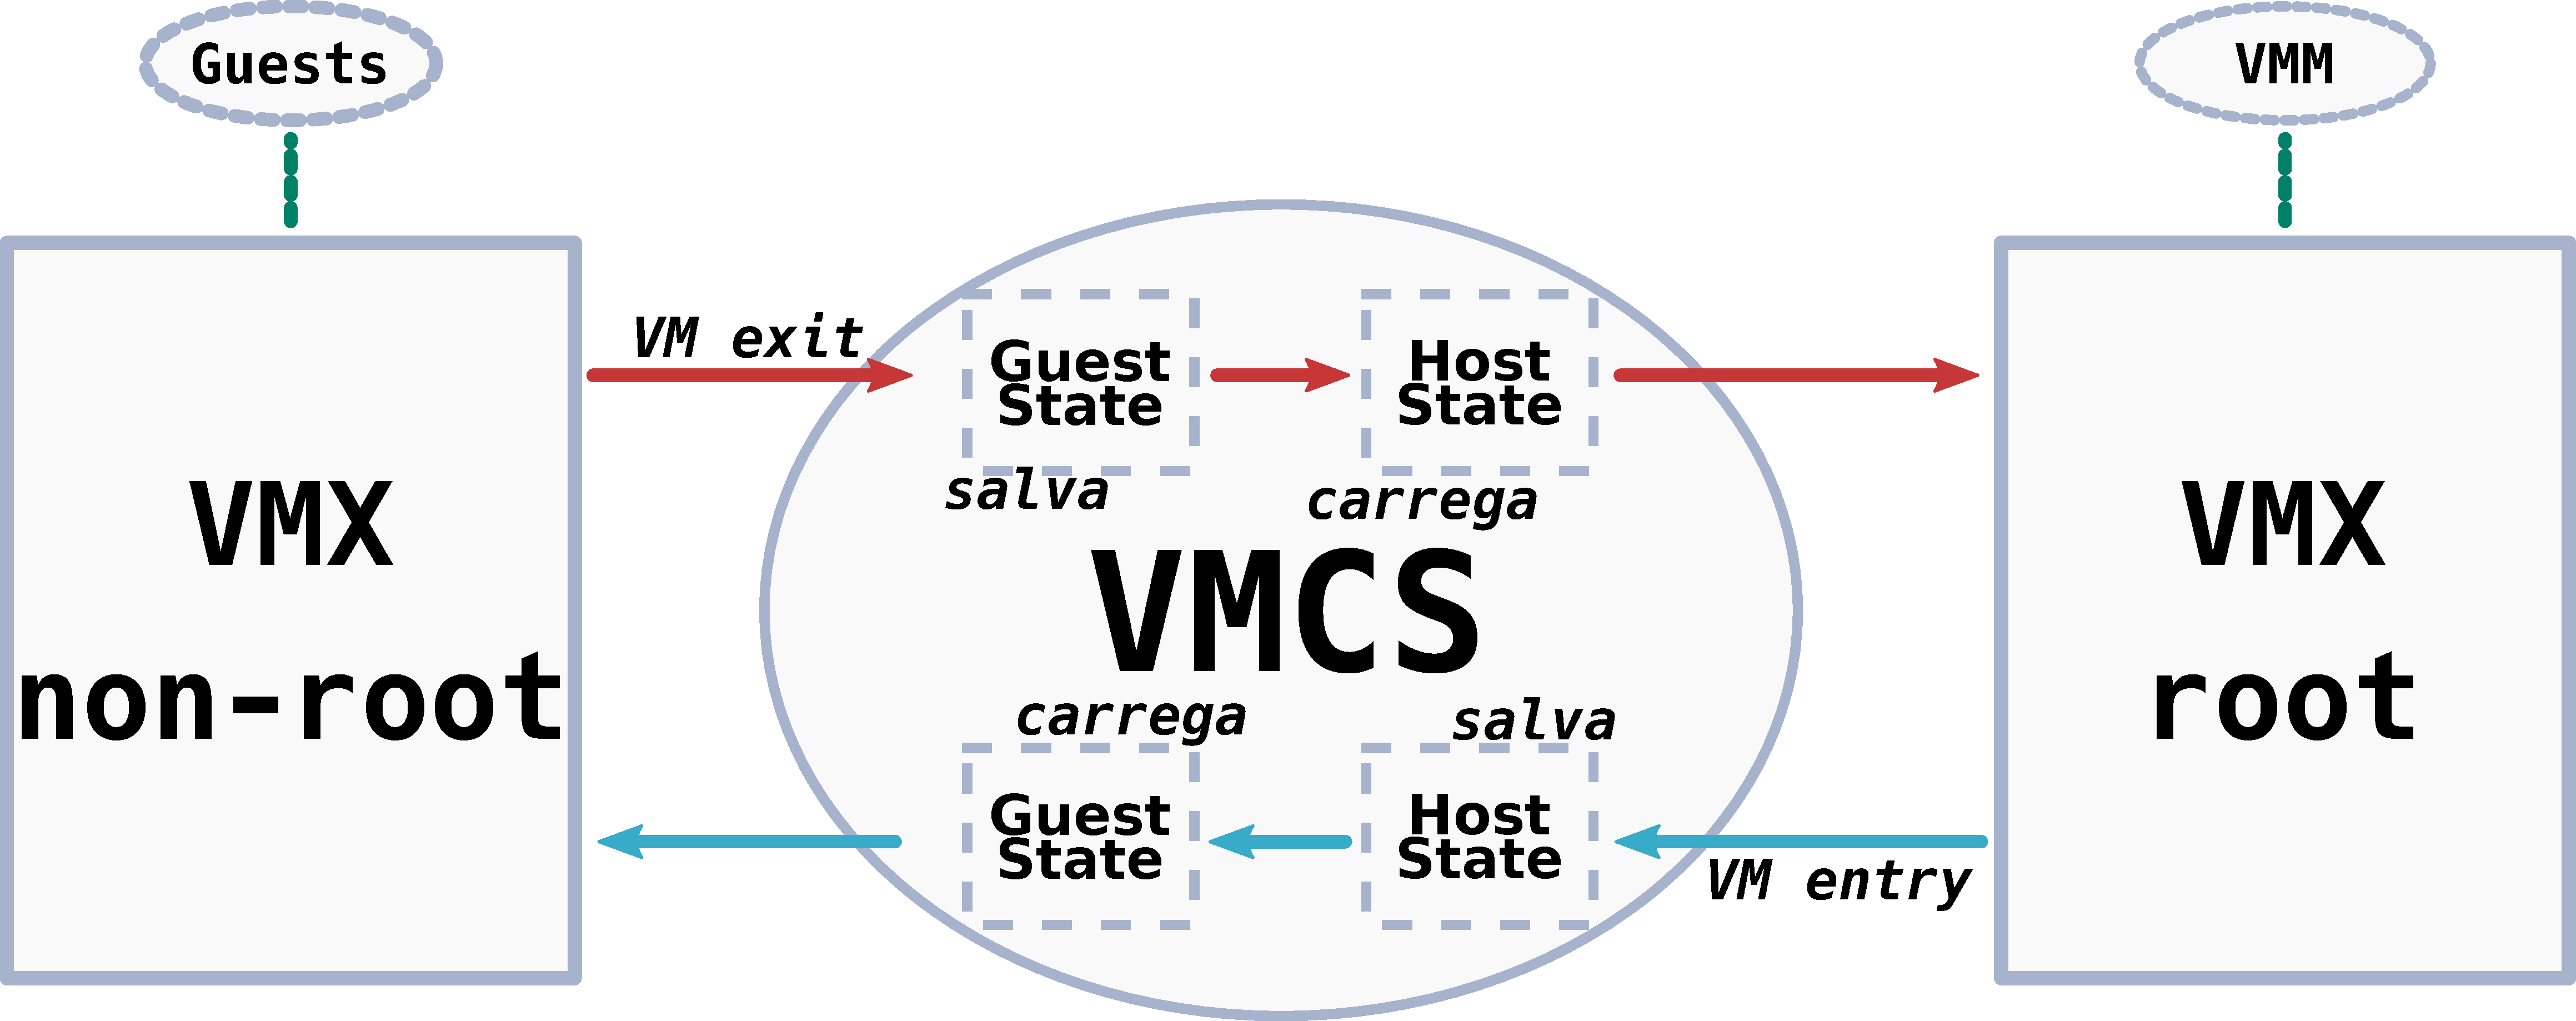
\includegraphics[width=0.6\textwidth]{vt-x_flow} 
  \caption{Fluxo do comportamento da tecnologia VT-x}
  \label{fig:vt-x_flow}
\end{figure}

O \emph{VMX non-root} é o modo de operação na qual a máquina \emph{guest}
executa, enquanto o \emph{VMX root} é o modo de operação utilizado pelo VMM. É
interessante observar que os dois modos tem suporte para os quatro níveis de
privilégios fornecidos pelos processadores Intel, isto permite que a máquina
\emph{guest} que tente executar uma instrução privilégiada em algum desses
nível forneçam tal informação para o VMM. Contudo, os software executando como
\emph{VMX non-root} são desprivilégiados de certa forma, a não pelo nível de
privilégios. Note da Figura \ref{fig:vt-x_flow} que existe uma trasição chamada
\emph{VM exit} e \emph{VM entry}. A transição \emph{VM exit} ocorre quando o
controle é transferido do \emph{guest} para o VMM, isto faz com que o estado da
máquina \emph{guest} seja salvo e o estado do \emph{host} seja carregado para
que o VMM decida como tratar a interrupção. No sentido oposto, ocorre a
transição \emph{VM entry} na qual o VMM transfere o controle para a máquina
\emph{guest}, para isto ela salva o estado do \emph{host} e carrega o estado
anterior do \emph{guest}. Todas as informações referentes a virtualização são
mantidas em uma estrutura de dados chamadas de \emph{virtual-machine control
structure (VMCS)} que basicamente tem por função gerenciar as transições entre
a \emph{VM entry} e \emph{VM exit}.


